
\addchap{Language sample and maps}
%%%
\subsubsection{Genus abbreviations (families)}
%%%
\begin{flushleft}
AB-AD=Abkhaz-Adyge, AUA=Austroasiatic, AUN=Austronesian, C-SUD=Central Sudanic, CHAD=Chadic, CHAP=Chapacura-Wanham, CHU=Chukotkan, CUSH=Cushitic, DRAV=Dravidian, ESK-A=Eskimo-Aleut, GUNW=Gunwingguan, HM-MI=Hmong-Mien, IE=Indo-European, IROQ=Iroquoian, KAMCH=Kamchatkan, KARTV=Kartvelian, KOIS=Koisan, KOM=Kombio, K-KRO=Kadugli-Krongo, MONG=Mongolic, MUSK=Muskogean, NA-DA=Nakh-Daghestanian, NA-DE=Na-Dene, NIG-C=Niger-Congo, NIL=Nilotic, S-BOU=South Bougainville, SE-RA=Lower Sepic-Ramu, SEM=Semitic, SIN-T=Sino-Tibetan, SONG=Songhai, TAI-K=Thai-Kadai, TANG=Tangkic, TUNG=Tungusic, TURK=Turkic, U-AZT=Uto-Aztecan, URAL=Uralic, YEN=Yeniseian, YUK=Yukagir
\end{flushleft}

\subsubsection{Genus abbreviations (branches and subbranches)}
%%%
\begin{flushleft}
5N=Five Nations, AAT=Avar-Andi-Tsezic, ABKH=Abhaz, ADYG=Adyge, ALBA=Albanian, ALT=Altay, ARAM=Aramaic, ARAP=Arapesh, ARME=Armenian, ATHA=Athabaskan, ATLA=Atlantic, BALT=Baltic, BANT=Bantoid, BE-CO=Benue-Congo, BRIT=Brittonic, BULG=Bulgar, BURM=Burmic, CELT=Celtic, CH-IN=Chechen-Ingush, CHIN=Chinese, CHUK=Chukchi, COM=Common, DARG=Dargwa, ENE=Enets, ENIN=Enindhilyagwa, ESKI=Eskimo, DAGH=Daghestanian, DAG=Dagur, FINN=Finnic, FOR=Formosan, GAE=Gaelic, GEOR=Georgian, GER=Germanic, GREE=Greek, HAUS=Hausa, HELL=Hellenic, HMON=Hmongic, HUNG=Hungarian, I-ARY=Indo-Aryan, I-IRA=Indo-Iranian, IRAN=Iranian, IT-W=Italo-Western, KARL=Karluk, KHAN=Khanty, KHOE=Khoekhoe, KIPCH=Kipchak, KORY=Koryak, KRON=Krongo, L-BUR=Lolo-Burmese, L-SEP-Lower Sepik, LEZG=Lezgian, LEND=Lendu, M-KH=Mon-Khmer, MAL-P=Malayo-Polynesian, MANCH=Manchu, MAND=Mande, MANS=Mansi, MOGH=Moghol, MONGO=Mongolian, MONGU=Monguor, MORD=Mordvin, NASI=Nasioi, NOU=Nanay-Orok-Ulcha, NENE=Nenets, NGAN=Nganasan, OCE=Oceanic, OR-UD=Oroch-Udege, OROM=Oromo, PERM=Permic,  REMB=Rembargic, ROM=Romance, S-WEL=South Wellesley, SAAM=Saamic, SAMO=Samoyedic, SAY=Sayan, SELK=Selkup, SIN=Sinitic, SLAV=Slavic, SUND=Sundic, TSO=Tsouic, VIET=Vietic, W-MP=Western Malayo-Polynesian, YEN=Yenisey, YI-KA=Yimas-Karawari, YOR=Yoruboid, YUP=Yupic
\end{flushleft}

\subsubsection{Geographic (sample) abbreviations}
%%%
\begin{flushleft}
EU=Europe, NA=North-Asia, NE=North-Eurasia, W=World
\end{flushleft}

\subsubsection{Type abbreviations}
%%%
\begin{flushleft}
ACAgr=Anti-construct state agreement, AConstr=Anti-construct state, AHDAgr=Appositive head-driven agreement, Constr=Construct state, DConstr=Double-construct state, HDAgr=Head-driven agreement, Inc=Adjective incorporation, Juxt=Juxtaposition, Link=Linker, MHPAgr=Modifier-headed possessor agreement, Nmlz=Attributive nominalization
\end{flushleft}

\begin{sidewaystable}
\begin{footnotesize}
\begin{tabular}{lll|l||ccc|c||l||ll}\label{sample}
\\%LATEX does not compile without this empty line
\hline\hline%\lsptoprule
\multicolumn{4}{c||}{Genealogical affiliation}&\multicolumn{4}{c||}{Geographic sampling}&Noun phrase type(s)&\\
\hline%\midrule
Family&\multicolumn{2}{l|}{(Sub-)Branch}&Language &EU&NA&NE&W &\#1/\#2(\#3)[\#4]&Reference\\
\hline%\midrule
\multicolumn{3}{l|}{	(Pidgin and creoles)	}					&	\textsc{	Berbice Dutch Creole	}	&	–	&	–	&	–	&	X	&	Juxt	&	\citealt{kouwenberg1994}	\\
{	AB-AD	}	&	ABKH	&		&	\textsc{	Abaza	}	&	X	&	–	&	–	&	–	&	HDAgr	&	\citealt{lomtatidze-etal1989}	\\
{	AB-AD	}	&	ABKH	&		&	\textsc{	Abkhaz	}	&	X	&	–	&	X	&	X	&	HDAgr	&	\citealt{chirikba2003}	\\
{	AB-AD	}	&	ADYG	&		&	\textsc{	Adyge (Abzakh)	}	&	X	&	–	&	–	&	–	&	Inc	&	\citealt{paris1989}	\\
{	AB-AD	}	&	ADYG	&		&	\textsc{	Karbardian	}	&	X	&	–	&	X	&	–	&	Inc	&	\citealt{colarusso2006}	\\
\multicolumn{3}{l|}{	AINU (isolate)	}					&	\textsc{	Ainu	}	&	–	&	X	&	X	&	X	&	Juxt	&	\citealt{refsing1986}	\\
{	AUA	}	&	M-KH	&	VIET	&	\textsc{	Vietnamese	}	&	–	&	–	&	–	&	X	&	Juxt	&	\citealt{nguyen1987}	\\
{	AUN	}	&	FOR	&	TSO	&	\textsc{	Tsou	}	&	–	&	–	&	–	&	X	&	AConstr	&	\citealt{szakos1994}	\\
{	AUN	}	&	MAL-P	&	OCE	&	\textsc{	Saliba	}	&	–	&	–	&	–	&	X	&	MHPAgr	&	\citealt{mosel1994}	\\
{	AUN	}	&	MAL-P	&	OCE	&	\textsc{	Takia	}	&	–	&	–	&	–	&	X	&	AConstr	&	\citealt{ross1998}	\\
{	AUN	}	&	WEMP	&	M-PH	&	\textsc{	Tagalog	}	&	–	&	–	&	–	&	X	&	Linker	&	\citealt{schachter1987}	\\
{	AUN	}	&	WEMP	&	SUND	&	\textsc{	Minangkabau	}	&	–	&	–	&	–	&	–	&	Juxt	&	\citealt{gil2005}	\\
\multicolumn{3}{l|}{	BASQUE (isolate)	}					&	\textsc{	Basque	}	&	X	&	–	&	X	&	X	&	Juxt	&	\citealt{hualde-etal2003}	\\
{	C-SUD	}	&	E	&	LEND	&	\textsc{	Ngiti	}	&	–	&	–	&	–	&	X	&	HDAgr/Juxt	&	\citealt{kutsch-lojenga1994}	\\
\multicolumn{3}{l|}{	CARIBAN	}					&	\textsc{	Hixkaryana	}	&	–	&	–	&	–	&	X	&	n.a.	&	\citealt{derbyshire1979}	\\
{	CHAD	}	&	W	&	HAUS	&	\textsc{	Hausa	}	&	–	&	–	&	–	&	X	&	ACAgr/HDAgr	&	\citealt{wolff1993}	\\
{	CHAP	}	&		&		&	\textsc{	Wari	}	&	–	&	–	&	–	&	X	&	MHPAgr	&	\citealt{everett-etal1997}	\\
{	CHU	}	&	CHUK	&		&	\textsc{	Chukchi	}	&	–	&	X	&	X	&	X	&	Inc/HDAgr	&	\citealt{skorik1960}	\\
{	CHU	}	&	KORY	&		&	\textsc{	Alutor	}	&	–	&	X	&	–	&	–	&	Inc/HDAgr	&	\citealt{nagayama2003}	\\
{	CHU	}	&	KORY	&		&	\textsc{	Koryak	}	&	–	&	X	&	X	&	–	&	Inc	&	\citealt{zukova1997}	\\
{	CUSH	}	&	E	&	OROM	&	\textsc{	Oromo (Boraana)	}	&	–	&	–	&	–	&	X	&	HDAgr	&	\citealt{stroomer1995}	\\
{	DRAV	}	&	S	&		&	\textsc{	Tamil	}	&	–	&	–	&	–	&	X	&	Juxt	&	\citealt{asher1982}	\\
{	ESK-A	}	&	ESKI	&	YUP	&	\textsc{	Yupic (Siberian)	}	&	–	&	X	&	X	&	–	&	Inc	&	\citealt{de-reuse1994}	\\
{	ESK-A	}	&	ESKI	&		&	\textsc{	Greenlandic (West)	}	&	–	&	–	&	–	&	X	&	HDAgr	&	\citealt{fortescue1984}	\\
{	GUNW	}	&	REMB	&		&	\textsc{	Ngalakan	}	&	–	&	–	&	–	&	X	&	HDAgr/Juxt	&	\citealt{merlan1983}	\\
{	HM-MI	}	&	HMON	&		&	\textsc{	Hmong Njua	}	&	–	&	–	&	–	&	X	&	Juxt	&	\citealt{harriehausen1990}	\\
{	IE	}	&	ALBA	&		&	\textsc{	Albanian	}	&	X	&	–	&	X	&	X	&	HDAgr/Nmlz+HDAgr	&	\citealt{demiraj1998}	\\
{	IE	}	&	ALBA	&		&	\textsc{	Arvanitika	}	&	X	&	–	&	–	&	–	&	HDAgr/Nmlz+HDAgr	&	\citealt{sasse1991}	\\
{	IE	}	&	ARME	&		&	\textsc{	Armenian (Eastern)	}	&	X	&	–	&	X	&	–	&	HDAgr/Juxt	&	\citealt{ajello1998}	\\
{	IE	}	&	BALT	&	E	&	\textsc{	Latvian	}	&	X	&	–	&	X	&	–	&	ACAgr/HDAgr	&	\citealt{nau1996}	\\
\hline\hline%\lspbottomrule
\end{tabular}
\end{footnotesize}
\end{sidewaystable}

\begin{sidewaystable}
\begin{footnotesize}
\begin{tabular}{lll|l||ccc|c||l||ll}\label{sample}
\\%LATEX does not compile without this empty line
\hline\hline%\lsptoprule
\multicolumn{4}{c||}{Genealogical affiliation}&\multicolumn{4}{c||}{Geographic sampling}&Noun phrase type(s)&\\
\hline%\midrule
Family&\multicolumn{2}{l|}{(Sub-)Branch}&Language &EU&NA&NE&W &\#1/\#2(\#3)[\#4]&Reference\\
\hline%\midrule
{	IE	}	&	BALT	&	E	&	\textsc{	Lithuanian	}	&	X	&	–	&	–	&	–	&	ACAgr/HDAgr	&	\citealt{press2005}	\\
{	IE	}	&	CELT	&	BRIT	&	\textsc{	Breton	}	&	X	&	–	&	–	&	–	&	HDAgr	&	
\citealt{ternes1992}	\\
{	IE	}	&	CELT	&	BRIT	&	\textsc{	Cornish	}	&	X	&	–	&	–	&	–	&	HDAgr	&	\citealt{thomas1992b}	\\
{	IE	}	&	CELT	&	BRIT	&	\textsc{	Welsh	}	&	X	&	–	&	X	&	–	&	HDAgr	&	\citealt{thomas1992a}	\\
{	IE	}	&	CELT	&	GAE	&	\textsc{	Gaelic (Scots)	}	&	X	&	–	&	X	&	–	&	HDAgr	&	\citealt{macauley1992}	\\
{	IE	}	&	CELT	&	GAE	&	\textsc{	Irish	}	&	X	&	–	&	–	&	–	&	HDAgr	&	\citealt{odochartaigh1992}	\\
{	IE	}	&	CELT	&	GAE	&	\textsc{	Manx	}	&	X	&	–	&	X	&	–	&	HDAgr/Juxt	&	\citealt{phillips2004}	\\
{	IE	}	&	GER	&	N	&	\textsc{	Danish	}	&	X	&	–	&	–	&	–	&	HDAgr[Nmlz]	&	own knowledge	\\
{	IE	}	&	GER	&	N	&	\textsc{	Danish (W-Jutlandic)	}	&	–	&	–	&	–	&	–	&	HDAgr	&	\citealt{lund1932}	\\
{	IE	}	&	GER	&	N	&	\textsc{	Faroese	}	&	X	&	–	&	–	&	–	&	ACAgr+HDAgr/HDAgr[Nmlz]	&	\citealt{lockwood1955}	\\
{	IE	}	&	GER	&	N	&	\textsc{	Icelandic	}	&	X	&	–	&	X	&	–	&	HDAgr[Nmlz]	&	\citealt{kress1982}	\\
{	IE	}	&	GER	&	N	&	\textsc{	Norwegian	}	&	X	&	–	&	–	&	–	&	ACAgr+HDAgr/HDAgr[Nmlz]	&	own knowledge	\\
{	IE	}	&	GER	&	N	&	\textsc{	Swedish	}	&	X	&	–	&	X	&	–	&	ACAgr+HDAgr/HDAgr[Nmlz]	&	own knowledge	\\
{	IE	}	&	GER	&	N	&	\textsc{	Swedish (Västerbotten)	}	&	X	&	–	&	X	&	–	&	Inc/HDAgr	&	\citealt{astrom1893}	\\
{	IE	}	&	GER	&	W	&	\textsc{	Dutch	}	&	X	&	–	&	–	&	–	&	ACAgr[Nmlz]	&	\citealt{donaldson1997}	\\
{	IE	}	&	GER	&	W	&	\textsc{	English	}	&	X	&	–	&	X	&	X	&	Inc[Nmlz]	&	own knowledge	\\
{	IE	}	&	GER	&	W	&	\textsc{	Frisian (West)	}	&	X	&	–	&	–	&	–	&	ACAgr	&	\citealt{tiersma1985}	\\
{	IE	}	&	GER	&	W	&	\textsc{	German	}	&	X	&	–	&	X	&	–	&	ACAgr[Nmlz]	&	own knowledge	\\
{	IE	}	&	GER	&	W	&	\textsc{	German (Alemannic)	}	&	X	&	–	&	–	&	–	&	ACAgr	&	\citealt{reese2006}	\\
{	IE	}	&	GER	&	W	&	\textsc{	German (Low)	}	&	X	&	–	&	–	&	–	&	ACAgr	&	\citealt{matras-etal2003}	\\
{	IE	}	&	GER	&	W	&	\textsc{	Luxembourgeois	}	&	X	&	–	&	–	&	–	&	ACAgr	&	\citealt{schanen-etal2006}	\\
{	IE	}	&	GER	&	W	&	\textsc{	Yiddish (East)	}	&	X	&	–	&	–	&	–	&	ACAgr(Nmlz+HDAgr)	&	\citealt{katz1987}	\\
{	IE	}	&	HELL	&	GREE	&	\textsc{	Greek	}	&	X	&	–	&	X	&	X	&	HDAgr(Nmlz+HDAgr)	&	\citealt{ruge1986}	\\
{	IE	}	&	I-IRA	&	I-ARY	&	\textsc{	Parya	}	&	–	&	X	&	X	&	–	&	ACAgr/Juxt	&	\citealt{oranskaja2001}	\\
{	IE	}	&	I-IRA	&	I-ARY	&	\textsc{	Romany (Burgenland)	}	&	X	&	–	&	X	&	–	&	HDAgr(Nmlz+HDAgr)	&	\citealt{halwachs-etal2002}	\\
{	IE	}	&	I-IRA	&	I-ARY	&	\textsc{	Romany (Doplenjska)	}	&	X	&	–	&	–	&	–	&	HDAgr	&	\citealt{cech2006}	\\
{	IE	}	&	I-IRA	&	I-ARY	&	\textsc{	Romany (Lithuanian)	}	&	X	&	–	&	–	&	–	&	HDAgr	&	\citealt{tenser2005}	\\
{	IE	}	&	I-IRA	&	I-ARY	&	\textsc{	Romany (Sepecides)	}	&	X	&	–	&	–	&	–	&	HDAgr	&	\citealt{cech-etal2003}	\\
{	IE	}	&	I-IRA	&	I-ARY	&	\textsc{	Romany (Sinte)	}	&	X	&	–	&	–	&	–	&	HDAgr	&	\citealt{holzinger1995}	\\
{	IE	}	&	I-IRA	&	IRAN	&	\textsc{	Kurmanjî	}	&	X	&	–	&	–	&	–	&	Constr	&	\citealt{aygen2007}	\\
\hline\hline%\lspbottomrule
\end{tabular}
\end{footnotesize}
\end{sidewaystable}

\begin{sidewaystable}
\begin{footnotesize}
\begin{tabular}{lll|l||ccc|c||l||ll}\label{sample}
\\%LATEX does not compile without this empty line
\hline\hline%\lsptoprule
\multicolumn{4}{c||}{Genealogical affiliation}&\multicolumn{4}{c||}{Geographic sampling}&Noun phrase type(s)&\\
\hline%\midrule
Family&\multicolumn{2}{l|}{(Sub-)Branch}&Language &EU&NA&NE&W &\#1/\#2(\#3)[\#4]&Reference\\
\hline%\midrule
{	IE	}	&	I-IRA	&	IRAN	&	\textsc{	Ossetic	}	&	X	&	–	&	X	&	–	&	Juxt(Constr)	&	\citealt{abaev1964}	\\
{	IE	}	&	I-IRA	&	IRAN	&	\textsc{	Persian	}	&	–	&	–	&	–	&	X	&	Constr	&	\citealt{mahootian1997}	\\
{	IE	}	&	I-IRA	&	IRAN	&	\textsc{	Roshanī	}	&	–	&	X	&	–	&	–	&	AConstr(Constr)	&	\citealt{payne1989}	\\
{	IE	}	&	I-IRA	&	IRAN	&	\textsc{	Shughnī	}	&	–	&	X	&	–	&	–	&	HDAgr	&	\citealt{payne1989}	\\
{	IE	}	&	I-IRA	&	IRAN	&	\textsc{	Tajik	}	&	–	&	X	&	X	&	–	&	Constr	&	\citealt{ido2005}	\\
{	IE	}	&	I-IRA	&	IRAN	&	\textsc{	Talysh (Northern)	}	&	X	&	–	&	X	&	–	&	AConstr	&	\citealt{schulze2000}	\\
{	IE	}	&	I-IRA	&	IRAN	&	\textsc{	Tati	}	&	X	&	–	&	–	&	–	&	Constr	&	\citealt{dzidalaev2000}	\\
{	IE	}	&	I-IRA	&	IRAN	&	\textsc{	Yazghūlāmī	}	&	–	&	X	&	X	&	–	&	HDAgr	&	\citealt{payne1989}	\\
{	IE	}	&	ROM	&	E	&	\textsc{	Rumanian (Daco)	}	&	X	&	–	&	X	&	–	&	HDAgr(Nmlz+HDAgr)	&	\citealt{beyer-etal1987}	\\
{	IE	}	&	ROM	&	IT-W	&	\textsc{	French	}	&	X	&	–	&	–	&	–	&	HDAgr	&	\citealt{harris1997}	\\
{	IE	}	&	ROM	&	IT-W	&	\textsc{	Galician	}	&	X	&	–	&	–	&	–	&	HDAgr	&	\citealt{perez-bouza1996}	\\
{	IE	}	&	ROM	&	IT-W	&	\textsc{	Italian	}	&	X	&	–	&	X	&	X	&	HDAgr	&	\citealt{maiden-etal2000}	\\
{	IE	}	&	ROM	&	IT-W	&	\textsc{	Portuguese	}	&	X	&	–	&	–	&	–	&	HDAgr	&	\citealt{gartner1998}	\\
{	IE	}	&	ROM	&	IT-W	&	\textsc{	Romansch	}	&	X	&	–	&	–	&	–	&	HDAgr	&	\citealt{haiman1997}	\\
{	IE	}	&	ROM	&	IT-W	&	\textsc{	Spanish (Castilian)	}	&	X	&	–	&	–	&	–	&	HDAgr	&	\citealt{torrego1998}	\\
{	IE	}	&	ROM	&	IT-W	&	\textsc{	Spanish (Catalan)	}	&	X	&	–	&	–	&	–	&	HDAgr	&	\citealt{hualde1992}	\\
{	IE	}	&	ROM	&	S	&	\textsc{	Corsican	}	&	X	&	–	&	–	&	–	&	HDAgr	&	\citealt{giacomo-marcellesi1997}	\\
{	IE	}	&	ROM	&	S	&	\textsc{	Sardinian	}	&	X	&	–	&	X	&	–	&	HDAgr	&	\citealt{jones1997}	\\
{	IE	}	&	SLAV	&	E	&	\textsc{	Belorussian	}	&	X	&	–	&	–	&	–	&	HDAgr	&	\citealt{mayo1993}	\\
{	IE	}	&	SLAV	&	E	&	\textsc{	Russian	}	&	X	&	–	&	X	&	X	&	ACAgr	&	own knowledge	\\
{	IE	}	&	SLAV	&	E	&	\textsc{	Ukrainian	}	&	X	&	–	&	X	&	–	&	HDAgr	&	\citealt{shevelov1993}	\\
{	IE	}	&	SLAV	&	S	&	\textsc{	Bulgarian	}	&	X	&	–	&	X	&	–	&	HDAgr	&	own knowledge	\\
{	IE	}	&	SLAV	&	S	&	\textsc{	Macedonian	}	&	X	&	–	&	–	&	–	&	HDAgr	&	\citealt{friedman2002}	\\
{	IE	}	&	SLAV	&	S	&	\textsc{	Serbo-Croatian	}	&	X	&	–	&	–	&	–	&	HDAgr(ACAgr)	&	\citealt{kordic1997}	\\
{	IE	}	&	SLAV	&	S	&	\textsc{	Slovene	}	&	X	&	–	&	–	&	–	&	HDAgr(ACAgr)[Nmlz+HDAgr]	&	\citealt{priestly1993}	\\
{	IE	}	&	SLAV	&	W	&	\textsc{	Czech	}	&	X	&	–	&	–	&	–	&	HDAgr	&	\citealt{janda-etal2000}	\\
{	IE	}	&	SLAV	&	W	&	\textsc{	Kashubian	}	&	X	&	–	&	–	&	–	&	HDAgr	&	\citealt{stone1993b}	\\
{	IE	}	&	SLAV	&	W	&	\textsc{	Polish	}	&	X	&	–	&	–	&	–	&	HDAgr	&	\citealt{feldstein-etal2002}	\\
{	IE	}	&	SLAV	&	W	&	\textsc{	Slovak	}	&	X	&	–	&	–	&	–	&	HDAgr	&	\citealt{short1993b}	\\
{	IE	}	&	SLAV	&	W	&	\textsc{	Sorbian (Lower)	}	&	X	&	–	&	X	&	–	&	HDAgr	&	\citealt{stone1993a}	\\
\hline\hline%\lspbottomrule
\end{tabular}
\end{footnotesize}
\end{sidewaystable}

\begin{sidewaystable}
\begin{footnotesize}
\begin{tabular}{lll|l||ccc|c||l||ll}\label{sample}
\\%LATEX does not compile without this empty line
\hline\hline%\lsptoprule
\multicolumn{4}{c||}{Genealogical affiliation}&\multicolumn{4}{c||}{Geographic sampling}&Noun phrase type(s)&\\
\hline%\midrule
Family&\multicolumn{2}{l|}{(Sub-)Branch}&Language &EU&NA&NE&W &\#1/\#2(\#3)[\#4]&Reference\\
\hline%\midrule
{	IE	}	&	SLAV	&	W	&	\textsc{	Sorbian (Upper)	}	&	X	&	–	&	–	&	–	&	HDAgr	&	\citealt{schaarschmidt2004}	\\
{	IROQ	}	&	N	&	5N	&	\textsc{	Cayuga	}	&	–	&	–	&	–	&	X	&	Inc	&	\citealt{mithun-etal1982}	\\
\multicolumn{3}{l|}{	JAPANESE (isolate)	}					&	\textsc{	Japanese	}	&	–	&	X	&	X	&	X	&	AConstr/Juxt	&	\citealt{backhouse1984}	\\
{	K-KRO	}	&	KRON	&		&	\textsc{	Krongo	}	&	–	&	–	&	–	&	X	&	ACAgr	&	\citealt{reh1985}	\\
{	KAMCH	}	&	W	&		&	\textsc{	Itelmen	}	&	–	&	X	&	X	&	X	&	ACAgr	&	\citealt{georg-etal1999}	\\
{	KARTV	}	&	GEOR	&		&	\textsc{	Georgian	}	&	X	&	–	&	X	&	X	&	HDAgr/Juxt(AHDAgr)	&	\citealt{cherchi1999}	\\
{	KARTV	}	&	SVAN	&		&	\textsc{	Svan	}	&	X	&	–	&	X	&	–	&	HDAgr[Juxt]	&	\citealt{schmidt1991}	\\
{	KARTV	}	&	ZAN	&		&	\textsc{	Laz	}	&	X	&	–	&	X	&	–	&	Juxt(HDAgr)	&	\citealt{holisky1991}	\\
{	KARTV	}	&	ZAN	&		&	\textsc{	Mingrelian	}	&	X	&	–	&	–	&	–	&	Juxt(HDAgr)	&	\citealt{harris1991b}	\\
{	KOIS	}	&	C	&	KHOE	&	\textsc{	Nama	}	&	–	&	–	&	–	&	X	&	Juxt	&	\citealt{hagman1977}	\\
{	KOM	}	&	ARAP	&		&	\textsc{	Arapesh (Bukiyip)	}	&	–	&	–	&	–	&	X	&	Juxt	&	\citealt{conrad1991}	\\
\multicolumn{3}{l|}{	KOREAN (isolate)	}					&	\textsc{	Korean	}	&	–	&	X	&	X	&	X	&	AConstr	&	\citealt{martin-etal1969}	\\
\multicolumn{3}{l|}{	MAPUDUNGUN (isolate)	}					&	\textsc{	Mapudungun	}	&	–	&	–	&	–	&	X	&	ACAgr/Juxt	&	\citealt{zuniga2000}	\\
{	MONG	}	&	DAG	&		&	\textsc{	Dagur	}	&	–	&	X	&	X	&	–	&	Juxt	&	\citealt{tsumagari2003}	\\
{	MONG	}	&	MOGH	&		&	\textsc{	Moghol	}	&	–	&	X	&	–	&	X	&	Juxt	&	\citealt{weiers2003}	\\
{	MONG	}	&	MONGO	&		&	\textsc{	Buryat	}	&	–	&	X	&	–	&	–	&	Juxt	&	\citealt{skribnik2003}	\\
{	MONG	}	&	MONGO	&		&	\textsc{	Kalmyk	}	&	–	&	X	&	–	&	–	&	Juxt	&	\citealt{blasing2003}	\\
{	MONG	}	&	MONGO	&		&	\textsc{	Khalkha	}	&	–	&	X	&	X	&	X	&	Juxt	&	\citealt{svantesson2003}	\\
{	MONG	}	&	MONGO	&		&	\textsc{	Mongol (Khamnigan)	}	&	–	&	X	&	–	&	–	&	Juxt	&	\citealt{janhunen2005}	\\
{	MONG	}	&	MONGO	&		&	\textsc{	Oyrat	}	&	–	&	–	&	–	&	–	&	Juxt	&	\citealt{birtalan2003}	\\
{	MONG	}	&	MONGU	&		&	\textsc{	Mangghuer	}	&	–	&	–	&	–	&	–	&	Juxt	&	\citealt{slater2003}	\\
{	MUSK	}	&	E	&		&	\textsc{	Koasati	}	&	–	&	–	&	–	&	X	&	Nmlz	&	\citealt{kimball1991}	\\
{	NA-DA	}	&	DAGH	&	AAT	&	\textsc{	Akhvakh	}	&	X	&	–	&	–	&	–	&	HDAgr	&	\citealt{magomedbekova2000}	\\
{	NA-DA	}	&	DAGH	&	AAT	&	\textsc{	Andi	}	&	X	&	–	&	–	&	–	&	HDAgr	&	\citealt{saidova2000}	\\
{	NA-DA	}	&	DAGH	&	AAT	&	\textsc{	Avar	}	&	X	&	–	&	–	&	X	&	HDAgr(Juxt)	&	\citealt{alekseev-etal1997}	\\
{	NA-DA	}	&	DAGH	&	AAT	&	\textsc{	Bagvalal	}	&	X	&	–	&	–	&	–	&	HDAgr	&	\citealt{magomedova2000a}	\\
{	NA-DA	}	&	DAGH	&	AAT	&	\textsc{	Bezhta	}	&	X	&	–	&	–	&	–	&	HDAgr	&	\citealt{kibrik-etal2004}	\\
{	NA-DA	}	&	DAGH	&	AAT	&	\textsc{	Botlikh	}	&	–	&	–	&	–	&	–	&	HDAgr	&	\citealt{azaev2000}	\\
{	NA-DA	}	&	DAGH	&	AAT	&	\textsc{	Chamalal	}	&	X	&	–	&	–	&	–	&	HDAgr	&	\citealt{magomedova2004} 	\\
{	NA-DA	}	&	DAGH	&	AAT	&	\textsc{	Godoberi	}	&	X	&	–	&	X	&	–	&	HDAgr	&	\citealt{saidova2004}	\\
{	NA-DA	}	&	DAGH	&	AAT	&	\textsc{	Hinukh	}	&	X	&	–	&	–	&	–	&	HDAgr	&	\citealt{isakov-etal2004}	\\
\hline\hline%\lspbottomrule
\end{tabular}
\end{footnotesize}
\end{sidewaystable}

\begin{sidewaystable}
\begin{footnotesize}
\begin{tabular}{lll|l||ccc|c||l||ll}\label{sample}
\\%LATEX does not compile without this empty line
\hline\hline%\lsptoprule
\multicolumn{4}{c||}{Genealogical affiliation}&\multicolumn{4}{c||}{Geographic sampling}&Noun phrase type(s)&\\
\hline%\midrule
Family&\multicolumn{2}{l|}{(Sub-)Branch}&Language &EU&NA&NE&W &\#1/\#2(\#3)[\#4]&Reference\\
\hline%\midrule
{	NA-DA	}	&	DAGH	&	AAT	&	\textsc{	Hunzib	}	&	X	&	–	&	–	&	–	&	HDAgr	&	\citealt{van-den-berg1995}	\\
{	NA-DA	}	&	DAGH	&	AAT	&	\textsc{	Karata	}	&	X	&	–	&	–	&	–	&	HDAgr	&	\citealt{magomedbekova1971}	\\
{	NA-DA	}	&	DAGH	&	AAT	&	\textsc{	Tindi	}	&	X	&	–	&	–	&	–	&	HDAgr	&	\citealt{magomedova2000b}	\\
{	NA-DA	}	&	DAGH	&	AAT	&	\textsc{	Tsez	}	&	X	&	–	&	X	&	–	&	ACAgr/Juxt(Nmlz)	&	\citealt{alekseev-etal2004}	\\
{	NA-DA	}	&	DAGH	&	DARG	&	\textsc{	Dargwa	}	&	X	&	–	&	X	&	–	&	ACAgr(Juxt)	&	\citealt{isaev2004}	\\
{	NA-DA	}	&	DAGH	&	LAK	&	\textsc{	Lak	}	&	X	&	–	&	X	&	X	&	HDAgr(ACAgr)	&	\citealt{abdullaev2000}	\\
{	NA-DA	}	&	DAGH	&	LEZG	&	\textsc{	Agul	}	&	X	&	–	&	–	&	–	&	Juxt	&	\citealt{sauman1941}	\\
{	NA-DA	}	&	DAGH	&	LEZG	&	\textsc{	Archi	}	&	X	&	–	&	X	&	–	&	HDAgr	&	\citealt{kibrik1994a}	\\
{	NA-DA	}	&	DAGH	&	LEZG	&	\textsc{	Budukh	}	&	X	&	–	&	–	&	–	&	Juxt	&	\citealt{alekseev1994b}	\\
{	NA-DA	}	&	DAGH	&	LEZG	&	\textsc{	Khinalug	}	&	X	&	–	&	–	&	–	&	Juxt	&	\citealt{deseriev1959}	\\
{	NA-DA	}	&	DAGH	&	LEZG	&	\textsc{	Kryz	}	&	X	&	–	&	–	&	–	&	Juxt	&	\citealt{saadiev1994}	\\
{	NA-DA	}	&	DAGH	&	LEZG	&	\textsc{	Lezgi	}	&	X	&	–	&	X	&	X	&	Juxt	&	\citealt{haspelmath1993}	\\
{	NA-DA	}	&	DAGH	&	LEZG	&	\textsc{	Rutul	}	&	X	&	–	&	X	&	–	&	AConstr	&	\citealt{alekseev1994a}	\\
{	NA-DA	}	&	DAGH	&	LEZG	&	\textsc{	Tabasaran	}	&	X	&	–	&	X	&	–	&	HDAgr/Juxt	&	\citealt{kurbanov1986}	\\
{	NA-DA	}	&	DAGH	&	LEZG	&	\textsc{	Tsakhur	}	&	X	&	–	&	X	&	–	&	ACAgr/Juxt	&	\citealt{schulze1997}	\\
{	NA-DA	}	&	DAGH	&	LEZG	&	\textsc{	Udi	}	&	X	&	–	&	–	&	–	&	Juxt	&	\citealt{schulze-furhoff1994}	\\
{	NA-DA	}	&	NAGH	&	BATS	&	\textsc{	Bats	}	&	X	&	–	&	X	&	–	&	HDAgr	&	\citealt{holisky-etal1994}	\\
{	NA-DA	}	&	NAGH	&	CH-IN	&	\textsc{	Chechen	}	&	X	&	–	&	X	&	X	&	HDAgr	&	\citealt{nichols1994a}	\\
{	NA-DA	}	&	NAGH	&	CH-IN	&	\textsc{	Ingush	}	&	X	&	–	&	–	&	–	&	HDAgr	&	\citealt{nichols1994b}	\\
{	NA-DE	}	&	ATHA	&		&	\textsc{	Sarcee	}	&	–	&	–	&	–	&	X	&	Inc	&	\citealt{cook1984}	\\
{	NIG-C	}	&	ATLA	&	N	&	\textsc{	Fula (Gombe)	}	&	–	&	–	&	–	&	X	&	HDAgr	&	\citealt{arnott1970}	\\
{	NIG-C	}	&	ATLA	&	S	&	\textsc{	Kisi	}	&	–	&	–	&	–	&	–	&	HDAgr	&	\citealt{tucker1995}	\\
{	NIG-C	}	&	BE-CO	&	BANT	&	\textsc{	Babungo	}	&	–	&	–	&	–	&	–	&	HDAgr	&	\citealt{schaub1985}	\\
{	NIG-C	}	&	BE-CO	&	BANT	&	\textsc{	Sesotho	}	&	–	&	–	&	–	&	–	&	HDAgr	&	\citealt{guma1971}	\\
{	NIG-C	}	&	BE-CO	&	BANT	&	\textsc{	Swahili	}	&	–	&	–	&	–	&	X	&	HDAgr	&	\citealt{gromova-etal1995}	\\
{	NIG-C	}	&	BE-CO	&	YOR	&	\textsc{	Yoruba	}	&	–	&	–	&	–	&	X	&	Juxt	&	\citealt{bamgbose1966}	\\
{	NIG-C	}	&	MAND	&	W	&	\textsc{	Bambara	}	&	–	&	–	&	–	&	X	&	Juxt	&	\citealt{brauner1974}	\\
{	NIL	}	&	S	&		&	\textsc{	Endo	}	&	–	&	–	&	–	&	X	&	ACAgr+Nmlz	&	\citealt{zwarts2003}	\\
{	NIL	}	&	W	&	LWO	&	\textsc{	Lango	}	&	–	&	–	&	–	&	X	&	Nmlz	&	\citealt{noonan1992}	\\
\multicolumn{3}{l|}{	NIVKH (isolate)	}					&	\textsc{	Nivkh	}	&	–	&	X	&	X	&	X	&	HDAgr	&	\citealt{gruzdeva1998}	\\
\hline\hline%\lspbottomrule
\end{tabular}
\end{footnotesize}
\end{sidewaystable}

\begin{sidewaystable}
\begin{footnotesize}
\begin{tabular}{lll|l||ccc|c||l||ll}\label{sample}
\\%LATEX does not compile without this empty line
\hline\hline%\lsptoprule
\multicolumn{4}{c||}{Genealogical affiliation}&\multicolumn{4}{c||}{Geographic sampling}&Noun phrase type(s)&\\
\hline%\midrule
Family&\multicolumn{2}{l|}{(Sub-)Branch}&Language &EU&NA&NE&W &\#1/\#2(\#3)[\#4]&Reference\\
\hline%\midrule
{	S-BOU	}	&	NASI	&		&	\textsc{	Nasioi	}	&	–	&	–	&	–	&	X	&	ACAgr/Juxt	&	\citealt{rausch1912}	\\
{	SE-RA	}	&	L-SEP	&	YI-KA	&	\textsc{	Yimas	}	&	–	&	–	&	–	&	X	&	HDAgr	&	\citealt{foley1991}	\\
{	SEM	}	&	C	&	ARAM	&	\textsc{	Assyrian	}	&	X	&	–	&	X	&	–	&	HDAgr	&	\citealt{krotkoff1982}	\\
{	SEM	}	&	W	&	C	&	\textsc{	Arabic (Cypriote)	}	&	X	&	–	&	–	&	–	&	HDAgr	&	\citealt{borg1985}	\\
{	SEM	}	&	W	&	C	&	\textsc{	Arabic (Egyptian)	}	&	–	&	–	&	–	&	X	&	HDAgr	&	\citealt{gary-etal1982}	\\
{	SEM	}	&	W	&	C	&	\textsc{	Maltese	}	&	X	&	–	&	X	&	–	&	HDAgr	&	\citealt{borg-etal1996}	\\
{	SEM	}	&	W	&	S	&	\textsc{	Amharic	}	&	–	&	–	&	–	&	X	&	Juxt(ACAgr)	&	\citealt{leslau1995}	\\
{	SIN-T	}	&	L-BUR	&	BURM	&	\textsc{	Burmese	}	&	–	&	–	&	–	&	X	&	Juxt/Nmlz	&	\citealt{wheatley1987}	\\
{	SIN-T	}	&	L-BUR	&	LOLO	&	\textsc{	Lahu	}	&	–	&	–	&	–	&	–	&	Nmlz	&	\citealt{matisoff1973}	\\
{	SIN-T	}	&	SIN	&	CHIN	&	\textsc{	Dungan	}	&	–	&	X	&	X	&	–	&	Juxt[Nmlz]	&	\citealt{kalimov1968}	\\
{	SIN-T	}	&	SIN	&	CHIN	&	\textsc{	Mandarin	}	&	–	&	–	&	–	&	X	&	Nmlz(Juxt)	&	\citealt{li-etal1981}	\\
{	SONG	}	&	S	&		&	\textsc{	Koyra Chiini	}	&	–	&	–	&	–	&	X	&	AConstr	&	\citealt{heath1998}	\\
{	TAI-K	}	&	TAI	&		&	\textsc{	Nung	}	&	–	&	–	&	–	&	–	&	Juxt(Nmlz)	&	\citealt{saul-etal1980}	\\
{	TAI-K	}	&	TAI	&		&	\textsc{	Thai	}	&	–	&	–	&	–	&	X	&	Juxt	&	\citealt{hudak1987}	\\
{	TANG	}	&	S	&	S-WEL	&	\textsc{	Kayardild	}	&	–	&	–	&	–	&	X	&	HDAgr	&	\citealt{evans1995}	\\
\multicolumn{3}{l|}{	TIWI (isolate)	}					&	\textsc{	Tiwi	}	&	–	&	–	&	–	&	X	&	HDAgr	&	\citealt{osborne1974}	\\
{	TUNG	}	&	AMUR	&	NOU	&	\textsc{	Nanay	}	&	–	&	X	&	–	&	–	&	Juxt	&	\citealt{avrorin1968}	\\
{	TUNG	}	&	AMUR	&	NOU	&	\textsc{	Orok	}	&	–	&	X	&	X	&	–	&	HDAgr	&	\citealt{petrova1967}	\\
{	TUNG	}	&	AMUR	&	NOU	&	\textsc{	Ulcha	}	&	–	&	–	&	X	&	–	&	Juxt[Nmlz]	&	\citealt{sunik1985}	\\
{	TUNG	}	&	AMUR	&	OR-UD	&	\textsc{	Oroch	}	&	–	&	X	&	X	&	–	&	Juxt(MHPAgr)	&	\citealt{avrorin-etal1967}	\\
{	TUNG	}	&	AMUR	&	OR-UD	&	\textsc{	Udege	}	&	–	&	X	&	X	&	X	&	HDAgr/MHPAgr	&	\citealt{nikolaeva-etal2001}	\\
{	TUNG	}	&	MANCH	&		&	\textsc{	Manchu	}	&	–	&	X	&	X	&	–	&	Juxt	&	\citealt{avrorin2000}	\\
{	TUNG	}	&	N	&		&	\textsc{	Even	}	&	–	&	X	&	X	&	X	&	HDAgr(MHPAgr)	&	\citealt{malchukov1995}	\\
{	TUNG	}	&	N	&		&	\textsc{	Evenki	}	&	–	&	X	&	X	&	–	&	HDAgr/Juxt/Nmlz(MHPAgr)	&	\citealt{nedjalkov1997}	\\
{	TUNG	}	&	N	&		&	\textsc{	Negidal	}	&	–	&	X	&	X	&	–	&	Juxt	&	\citealt{nedalkov2001}	\\
{	TUNG	}	&	N	&		&	\textsc{	Solon	}	&	–	&	X	&	–	&	–	&	Juxt	&	\citealt{cincius1997}	\\
{	TURK	}	&	BULG	&		&	\textsc{	Chuvash	}	&	X	&	–	&	X	&	X	&	Juxt(Nmlz)	&	\citealt{clark1998a}	\\
{	TURK	}	&	COM	&	ALT	&	\textsc{	Altay (Southern)	}	&	–	&	X	&	X	&	–	&	Juxt	&	\citealt{baskakov1997b}	\\
{	TURK	}	&	COM	&	ALT	&	\textsc{	Kirghiz	}	&	–	&	X	&	–	&	–	&	Juxt	&	\citealt{kara2003}	\\
{	TURK	}	&	COM	&	KARL	&	\textsc{	Uygur	}	&	–	&	X	&	–	&	–	&	Juxt[Nmlz]	&	\citealt{nadzip1971}	\\
\hline\hline%\lspbottomrule
\end{tabular}
\end{footnotesize}
\end{sidewaystable}

\begin{sidewaystable}
\begin{footnotesize}
\begin{tabular}{lll|l||ccc|c||l||ll}\label{sample}
\\%LATEX does not compile without this empty line
\hline\hline%\lsptoprule
\multicolumn{4}{c||}{Genealogical affiliation}&\multicolumn{4}{c||}{Geographic sampling}&Noun phrase type(s)&\\
\hline%\midrule
Family&\multicolumn{2}{l|}{(Sub-)Branch}&Language &EU&NA&NE&W &\#1/\#2(\#3)[\#4]&Reference\\
\hline%\midrule
{	TURK	}	&	COM	&	KARL	&	\textsc{	Uzbek	}	&	–	&	X	&	X	&	–	&	Juxt[Nmlz]	&	\citealt{boeschoten1998}	\\
{	TURK	}	&	COM	&	KIPCH	&	\textsc{	Bashkir	}	&	–	&	X	&	–	&	–	&	Juxt	&	\citealt{poppe1964}	\\
{	TURK	}	&	COM	&	KIPCH	&	\textsc{	Karachay-Balkar	}	&	X	&	–	&	–	&	–	&	Juxt	&	\citealt{seegmiller1996}	\\
{	TURK	}	&	COM	&	KIPCH	&	\textsc{	Karaim	}	&	X	&	–	&	–	&	–	&	Juxt	&	\citealt{kocaoglu2006}	\\
{	TURK	}	&	COM	&	KIPCH	&	\textsc{	Karakalpak	}	&	–	&	X	&	–	&	–	&	Juxt	&	\citealt{baskakov2001}	\\
{	TURK	}	&	COM	&	KIPCH	&	\textsc{	Kazakh	}	&	–	&	X	&	X	&	–	&	Juxt	&	\citealt{kara2002}	\\
{	TURK	}	&	COM	&	KIPCH	&	\textsc{	Kumyk	}	&	X	&	–	&	–	&	–	&	Juxt	&	\citealt{kadyradziev2000}	\\
{	TURK	}	&	COM	&	KIPCH	&	\textsc{	Nogay	}	&	X	&	–	&	–	&	–	&	Juxt	&	\citealt{baskakov1940}	\\
{	TURK	}	&	COM	&	KIPCH	&	\textsc{	Tatar	}	&	X	&	–	&	–	&	–	&	Juxt	&	\citealt{poppe1963}	\\
{	TURK	}	&	COM	&	LENA	&	\textsc{	Dolgan	}	&	–	&	X	&	–	&	–	&	Juxt	&	\citealt{ubratova1985}	\\
{	TURK	}	&	COM	&	LENA	&	\textsc{	Sakha	}	&	–	&	X	&	X	&	–	&	Juxt	&	\citealt{krueger1962}	\\
{	TURK	}	&	COM	&	OGUZ	&	\textsc{	Azerbaijani	}	&	–	&	X	&	–	&	–	&	Juxt	&	\citealt{budagova1982}	\\
{	TURK	}	&	COM	&	OGUZ	&	\textsc{	Gagauz	}	&	X	&	–	&	–	&	–	&	Juxt	&	\citealt{pokrovskaja1997}	\\
{	TURK	}	&	COM	&	OGUZ	&	\textsc{	Turkish	}	&	X	&	–	&	X	&	X	&	Juxt[Nmlz]	&	\citealt{kornfilt1997}	\\
{	TURK	}	&	COM	&	OGUZ	&	\textsc{	Turkmen	}	&	–	&	X	&	–	&	–	&	Juxt	&	\citealt{clark1998b}	\\
{	TURK	}	&	COM	&	SAY	&	\textsc{	Tuvan	}	&	–	&	X	&	X	&	–	&	Juxt	&	\citealt{anderson-etal1999}	\\
{	TURK	}	&	COM	&	YEN	&	\textsc{	Khakaz	}	&	–	&	X	&	X	&	–	&	Juxt	&	\citealt{anderson1998}	\\
{	TURK	}	&	COM	&	YEN	&	\textsc{	Shor	}	&	–	&	X	&	–	&	–	&	Juxt	&	\citealt{donidze1997}	\\
{	U-AZT	}	&	N	&		&	\textsc{	Hopi (Toreva)	}	&	–	&	–	&	–	&	X	&	DConstr	&	\citealt{whorf1946}	\\
{	U-AZT	}	&	S	&		&	\textsc{	Pipil	}	&	–	&	–	&	–	&	X	&	HDAgr	&	\citealt{campbell-l1985}	\\
{	URAL	}	&	FINN	&		&	\textsc{	Estonian	}	&	X	&	–	&	–	&	–	&	HDAgr	&	\citealt{viitso1998}	\\
{	URAL	}	&	FINN	&		&	\textsc{	Finnish	}	&	X	&	–	&	X	&	X	&	HDAgr	&	\citealt{buchholz2004}	\\
{	URAL	}	&	FINN	&		&	\textsc{	Ingrian	}	&	X	&	–	&	–	&	–	&	HDAgr	&	\citealt{laanest1997}	\\
{	URAL	}	&	FINN	&		&	\textsc{	Karelian	}	&	X	&	–	&	–	&	–	&	HDAgr	&	\citealt{zajkov1999}	\\
{	URAL	}	&	FINN	&		&	\textsc{	Livonian	}	&	X	&	–	&	–	&	–	&	HDAgr	&	\citealt{moseley2002}	\\
{	URAL	}	&	FINN	&		&	\textsc{	Vepsian	}	&	X	&	–	&	–	&	–	&	HDAgr	&	\citealt{sajceva1981}	\\
{	URAL	}	&	FINN	&		&	\textsc{	Votian	}	&	X	&	–	&	–	&	–	&	HDAgr	&	\citealt{nikolaeva1997}	\\
{	URAL	}	&	HUNG	&		&	\textsc{	Hungarian	}	&	X	&	–	&	X	&	X	&	Juxt	&	\citealt{kenesei-etal1998}	\\
{	URAL	}	&	KHANT	&		&	\textsc{	Khanty (Northern)	}	&	–	&	X	&	X	&	–	&	Juxt	&	\citealt{nikolaeva1999}	\\
{	URAL	}	&	MANS	&		&	\textsc{	Mansi	}	&	–	&	X	&	X	&	–	&	Juxt	&	\citealt{riese2001}	\\
\hline\hline%\lspbottomrule
\end{tabular}
\end{footnotesize}
\end{sidewaystable}

\begin{sidewaystable}
\begin{footnotesize}
\begin{tabular}{lll|l||ccc|c||l||ll}\label{sample}
\\%LATEX does not compile without this empty line
\hline\hline%\lsptoprule
\multicolumn{4}{c||}{Genealogical affiliation}&\multicolumn{4}{c||}{Geographic sampling}&Noun phrase type(s)&\\
\hline%\midrule
Family&\multicolumn{2}{l|}{(Sub-)Branch}&Language &EU&NA&NE&W &\#1/\#2(\#3)[\#4]&Reference\\
\hline%\midrule
{	URAL	}	&	MARI	&		&	\textsc{	Mari (Hill)	}	&	X	&	–	&	X	&	–	&	Juxt[Nmlz+AHDAgr]	&	\citealt{alhoniemi1993}	\\
{	URAL	}	&	MARI	&		&	\textsc{	Mari (Meadow)	}	&	X	&	–	&	–	&	–	&	Juxt[Nmlz+AHDAgr]	&	\citealt{alhoniemi1993}	\\
{	URAL	}	&	MORD	&		&	\textsc{	Mordvin (Erzya)	}	&	X	&	–	&	X	&	–	&	Juxt	&	\citealt{zavodova1964}	\\
{	URAL	}	&	MORD	&		&	\textsc{	Mordvin (Moksha)	}	&	X	&	–	&	–	&	–	&	Juxt	&	\citealt{zavodova1964}	\\
{	URAL	}	&	PERM	&		&	\textsc{	Komi-Permyak	}	&	X	&	–	&	–	&	–	&	Juxt(Nmlz+AHDAgr)	&	\citealt{lytkin1966b}	\\
{	URAL	}	&	PERM	&		&	\textsc{	Komi-Zyrian	}	&	X	&	–	&	–	&	–	&	Juxt(Nmlz+AHDAgr)	&	\citealt{kokkonen1984}	\\
{	URAL	}	&	PERM	&		&	\textsc{	Udmurt	}	&	X	&	–	&	X	&	–	&	Juxt(Nmlz+AHDAgr)[AHDAgr]	&	\citealt{winkler2001}	\\
{	URAL	}	&	SAAM	&	E	&	\textsc{	Saami (Inari)	}	&	–	&	–	&	–	&	–	&	AConstr/Juxt	&	\citealt{olthuis2000}	\\
{	URAL	}	&	SAAM	&	E	&	\textsc{	Saami (Kildin)	}	&	X	&	–	&	–	&	–	&	AConstr/Juxt[HDrAgr]	&	own knowledge	\\
{	URAL	}	&	SAAM	&	E	&	\textsc{	Saami (Skolt)	}	&	–	&	–	&	–	&	–	&	AConstr/Juxt	&	own knowledge	\\
{	URAL	}	&	SAAM	&	E	&	\textsc{	Saami (Ter)	}	&	–	&	–	&	–	&	–	&	AConstr/Juxt	&	own knowledge	\\
{	URAL	}	&	SAAM	&	W	&	\textsc{	Saami (Lule)	}	&	–	&	–	&	–	&	–	&	AConstr/Juxt	&	\citealt{spiik1989}	\\
{	URAL	}	&	SAAM	&	W	&	\textsc{	Saami (Northern)	}	&	X	&	–	&	X	&	X	&	AConstr/DConstr/HDAgr/Juxt	&	own knowledge	\\
{	URAL	}	&	SAAM	&	W	&	\textsc{	Saami (Pite)	}	&	–	&	–	&	–	&	–	&	AConstr/Juxt	&	\citealt{lehtiranta1992}	\\
{	URAL	}	&	SAAM	&	W	&	\textsc{	Saami (South)	}	&	X	&	–	&	–	&	–	&	AConstr/Juxt	&	\citealt{bergsland1994}	\\
{	URAL	}	&	SAAM	&	W	&	\textsc{	Saami (Ume)	}	&	–	&	–	&	–	&	–	&	AConstr/Juxt	&	own knowledge	\\
{	URAL	}	&	SAMO	&	ENE	&	\textsc{	Enets (Forest)	}	&	–	&	X	&	X	&	–	&	Juxt	&	\citealt{kunnap1999}	\\
{	URAL	}	&	SAMO	&	NENE	&	\textsc{	Nenets (Tundra)	}	&	–	&	X	&	X	&	X	&	Juxt	&	\citealt{decsy1966}	\\
{	URAL	}	&	SAMO	&	NGAN	&	\textsc{	Nganasan	}	&	–	&	X	&	X	&	–	&	Juxt	&	\citealt{helimski1998a}	\\
{	URAL	}	&	SAMO	&	SELK	&	\textsc{	Selkup	}	&	–	&	X	&	X	&	–	&	Juxt	&	\citealt{helimski1998b}	\\
{	YEN	}	&	N	&		&	\textsc{	Ket	}	&	–	&	X	&	X	&	X	&	Juxt(HDAgr)[Nmlz]	&	\citealt{vajda2004}	\\
{	YUK	}	&		&		&	\textsc{	Yukagir (Kolyma)	}	&	–	&	X	&	–	&	–	&	AConstr/Inc	&	\citealt{maslova2003b}	\\
{	YUK	}	&		&		&	\textsc{	Yukagir (Tundra)	}	&	–	&	X	&	X	&	X	&	AConstr/Inc	&	\citealt{maslova2003a}	\\
\hline\hline%\lspbottomrule
\end{tabular}
\end{footnotesize}
\end{sidewaystable}

\newpage
\begin{sidewaysfigure}
    \begin{minipage}[b][8cm][c]{2\baselineskip}
        \caption[Adjective attribution marking, World]{Adjective attribution marking in the world's languages; (unbalanced) sample of 71 languages}
    \end{minipage}
%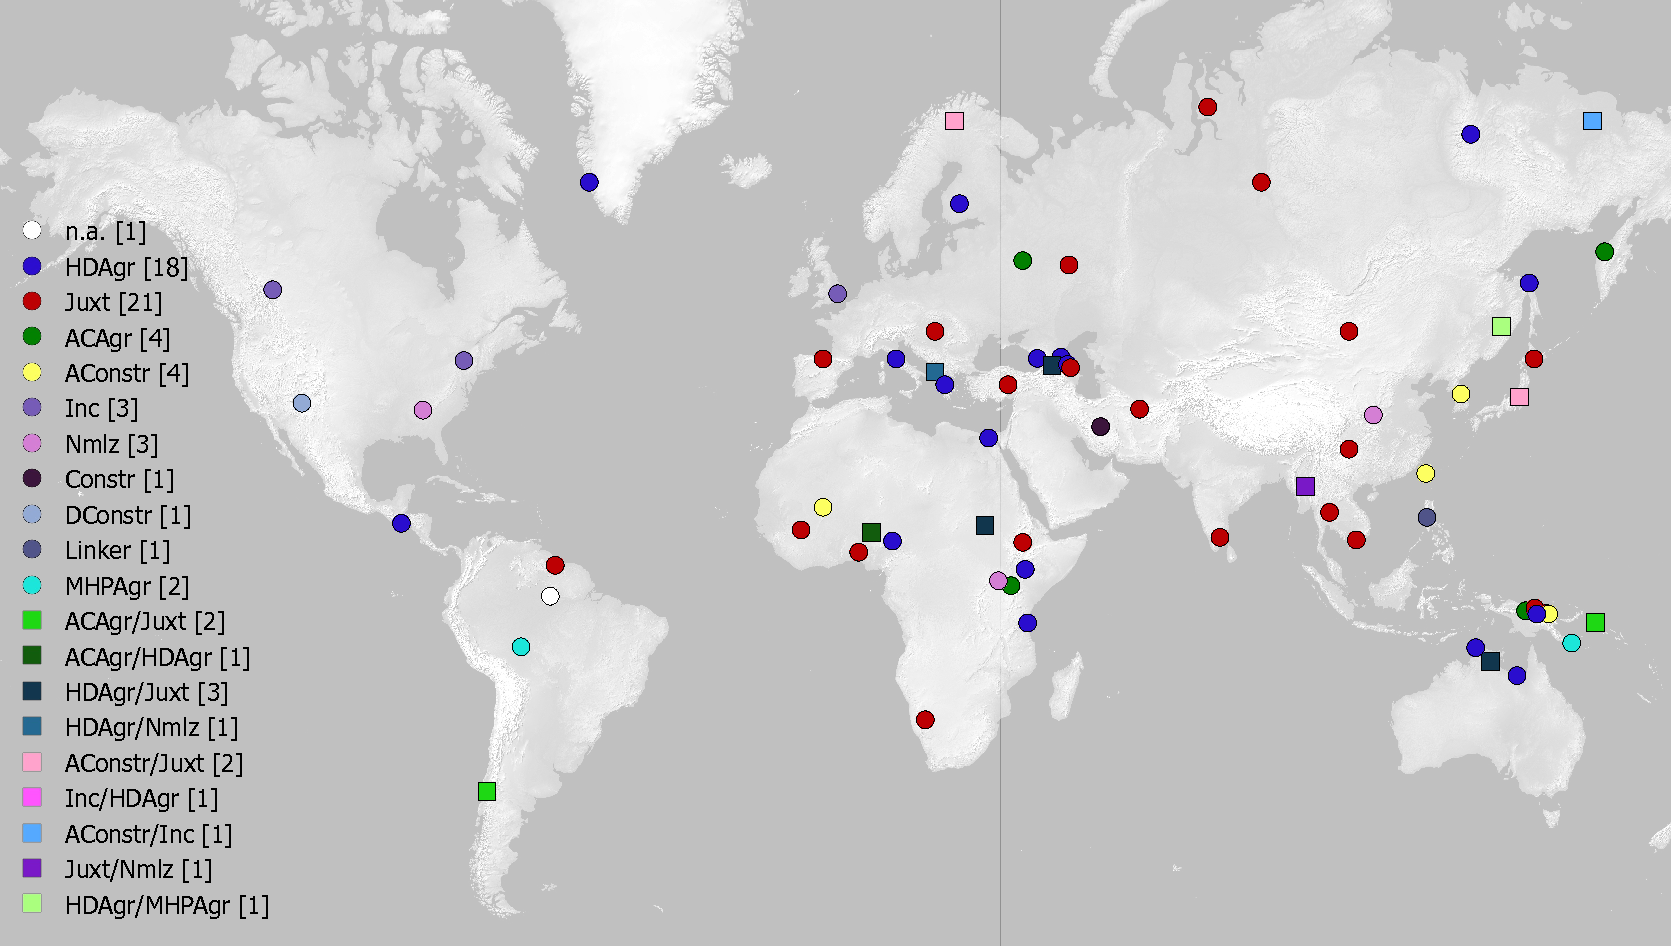
\includegraphics[width=\textheight,angle=90]{WorldMap.jpg}
\label{WorldMap}
\end{sidewaysfigure}

\newpage
\begin{sidewaysfigure}
    \begin{minipage}[b][8cm][c]{2\baselineskip}
        \caption[Adjective attribution marking, World, main types]{Adjective attribution marking in the world's languages; (unbalanced) sample of 71 languages coded for main morpho-syntactic types}
    \end{minipage}
%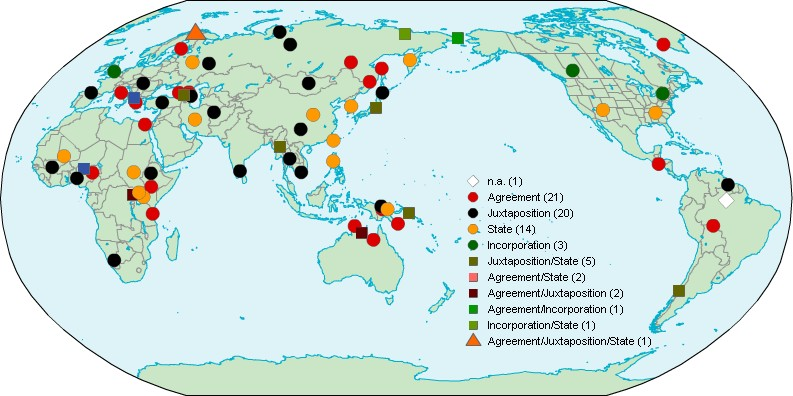
\includegraphics[width=\textheight,angle=90]{WorldMapTyp.jpg}
\label{WorldMapTyp}
\end{sidewaysfigure}

\newpage
\begin{sidewaysfigure}
    \begin{minipage}[b][8cm][c]{2\baselineskip}
        \caption[Adjective attribution marking, North-Eurasia]{Adjective attribution marking in the languages of North-Eurasia; 85 languages representing all genera of the area}
    \end{minipage}
%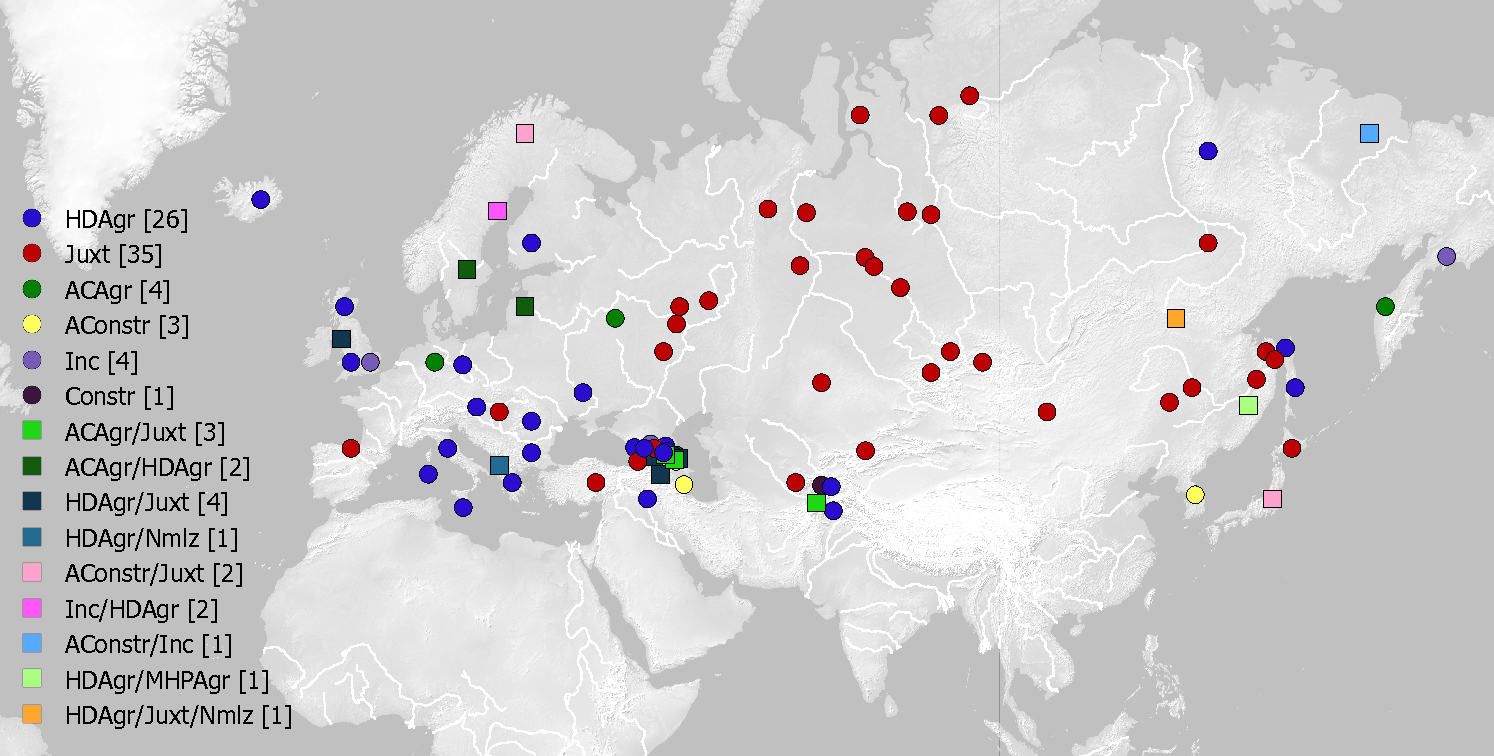
\includegraphics[width=\textheight,angle=90]{NEMap.jpg}
\label{NEMap}
\end{sidewaysfigure}

\newpage
\begin{sidewaysfigure}
    \begin{minipage}[b][8cm][c]{2\baselineskip}
        \caption[Adjective attribution marking, North-Eurasia, main types]{Adjective attribution marking in the languages of North-Eurasia; 85 languages representing all genera of the area coded for main morpho-syntactic types}
    \end{minipage}
%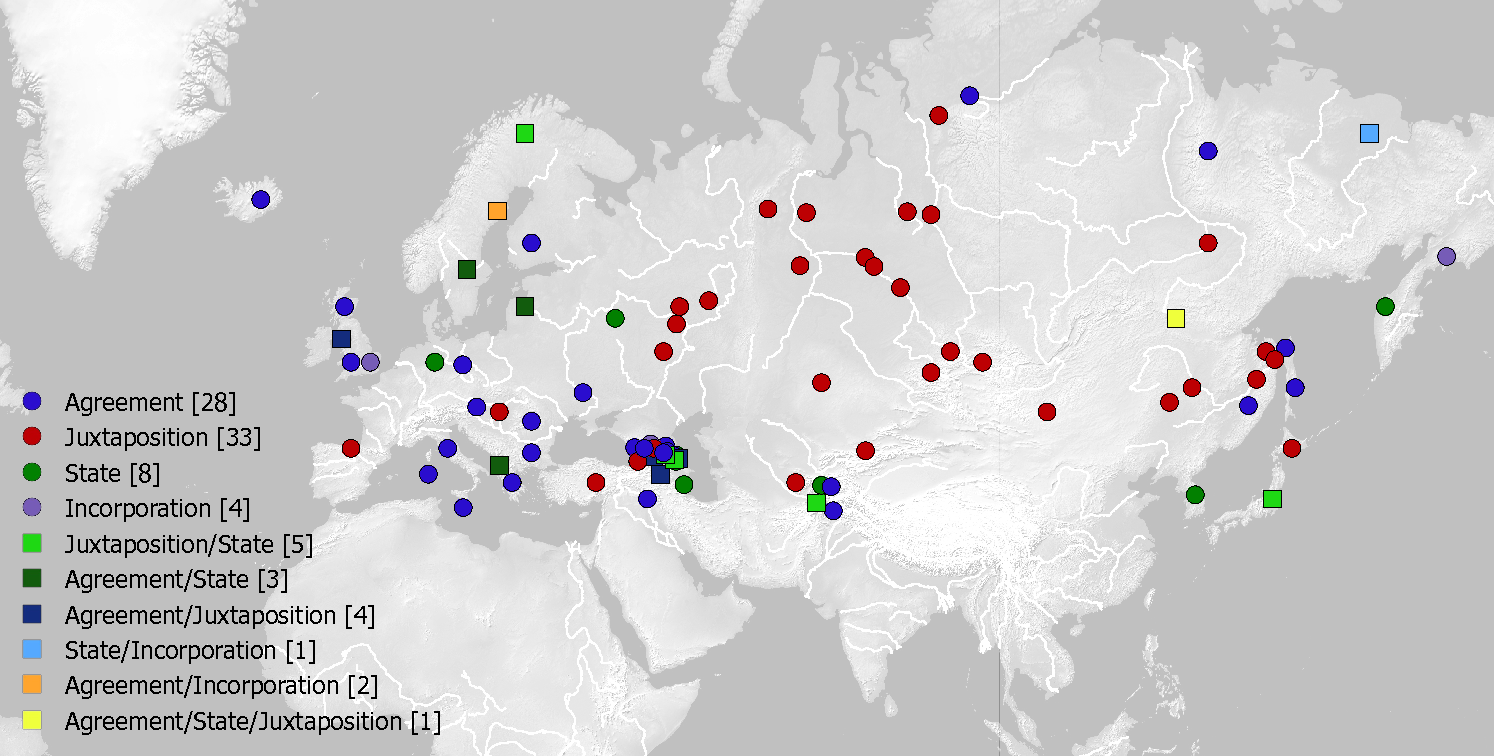
\includegraphics[width=\textheight,angle=90]{NEMapTyp.jpg}
\label{NEMapTyp}
\end{sidewaysfigure}

\newpage
\begin{sidewaysfigure}
    \begin{minipage}[b][8cm][c]{2\baselineskip}
        \caption[Adjective attribution marking, North-Asia]{Adjective attribution marking in the languages of North-Asia; 53 languages}
    \end{minipage}
%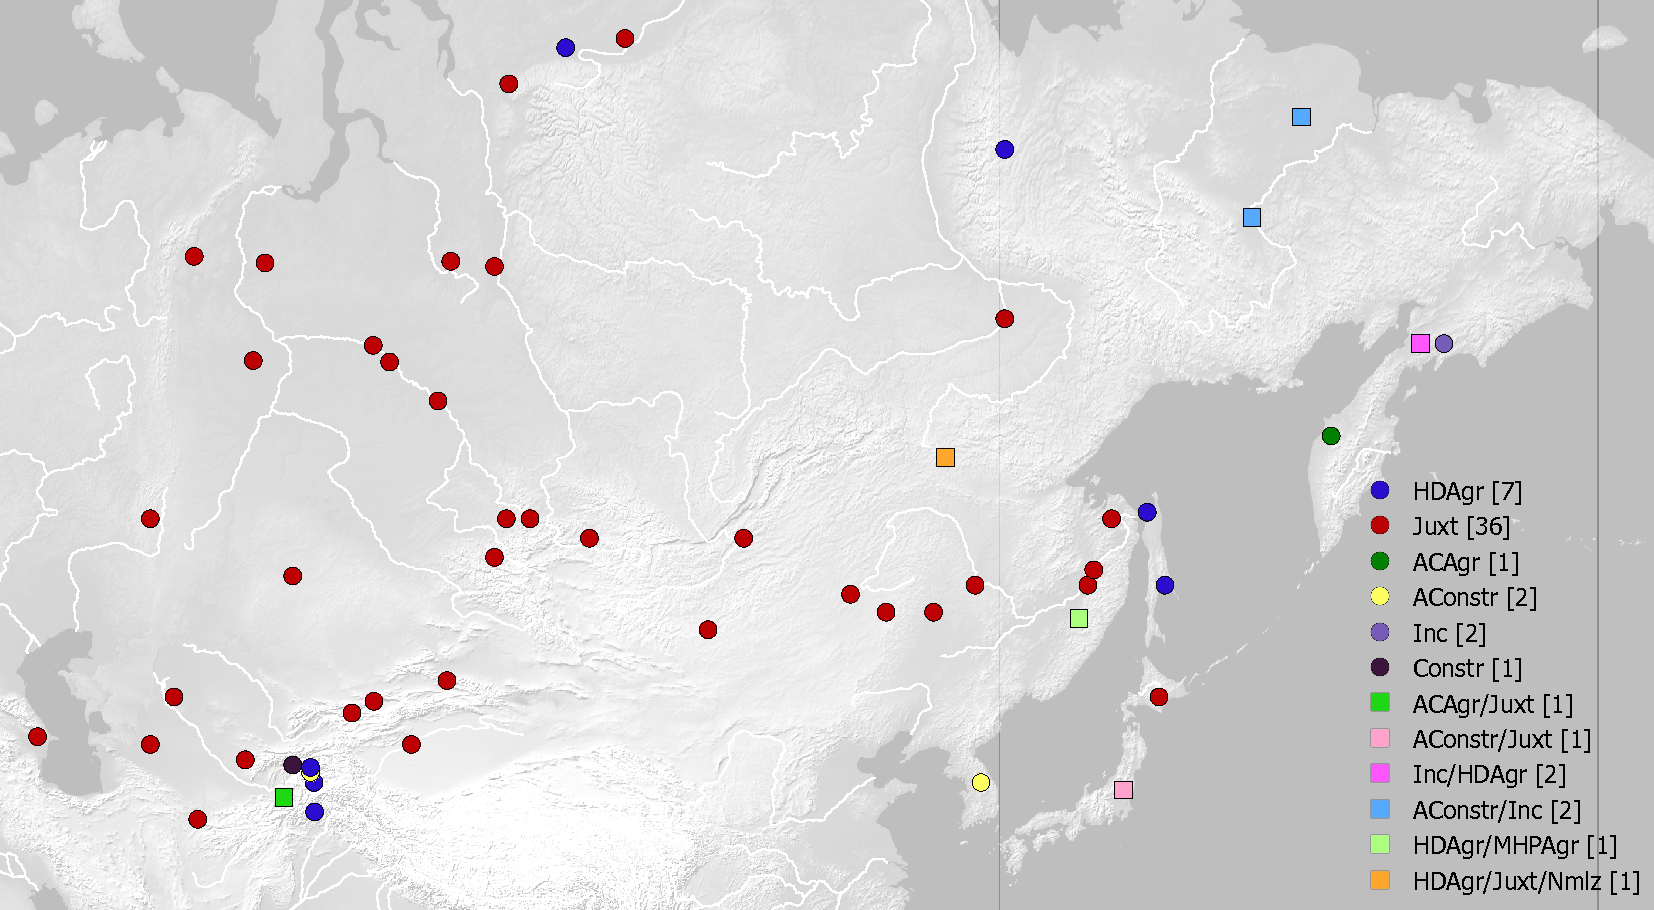
\includegraphics[width=\textheight,angle=90]{NAMap.jpg}
\label{NAMap}
\end{sidewaysfigure}

\newpage
\begin{sidewaysfigure}
    \begin{minipage}[b][8cm][c]{2\baselineskip}
        \caption[Adjective attribution marking, North-Asia, main types]{Adjective attribution marking in the languages of North-Asia; 53 languages coded for main morpho-syntactic types}
    \end{minipage}
%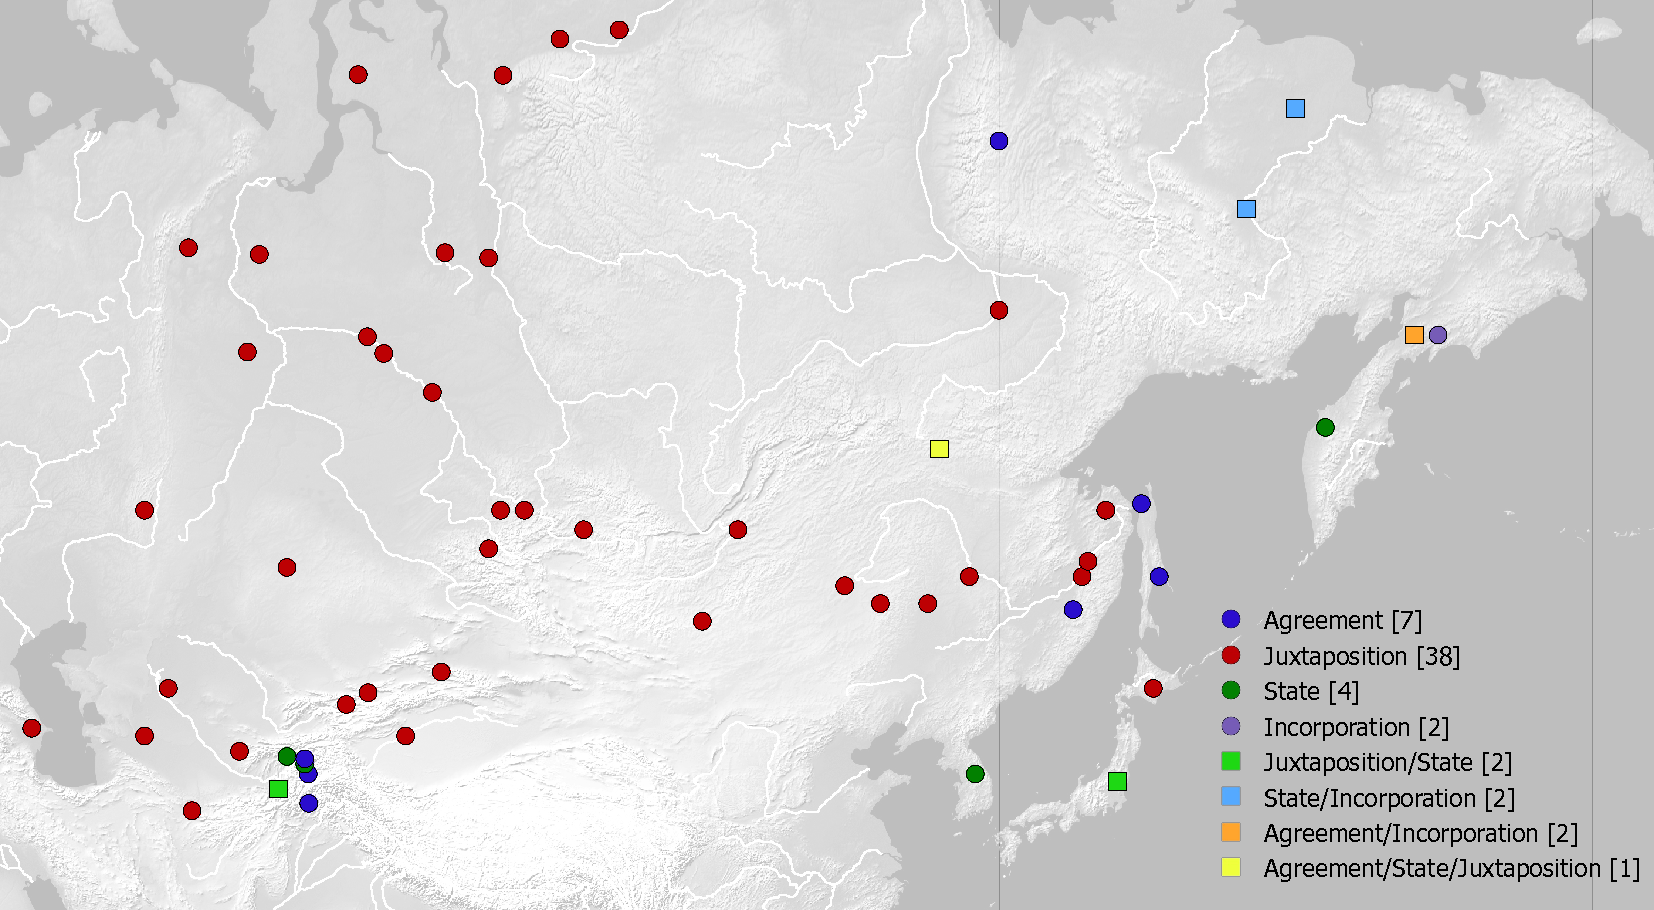
\includegraphics[width=\textheight,angle=90]{NAMapTyp.jpg}
\label{NAMapTyp}
\end{sidewaysfigure}

\newpage
\begin{sidewaysfigure}
    \begin{minipage}[b][8cm][c]{2\baselineskip}
        \caption[Adjective attribution marking, Europe]{Adjective attribution marking in the languages of Europe; 123 languages}
    \end{minipage}
%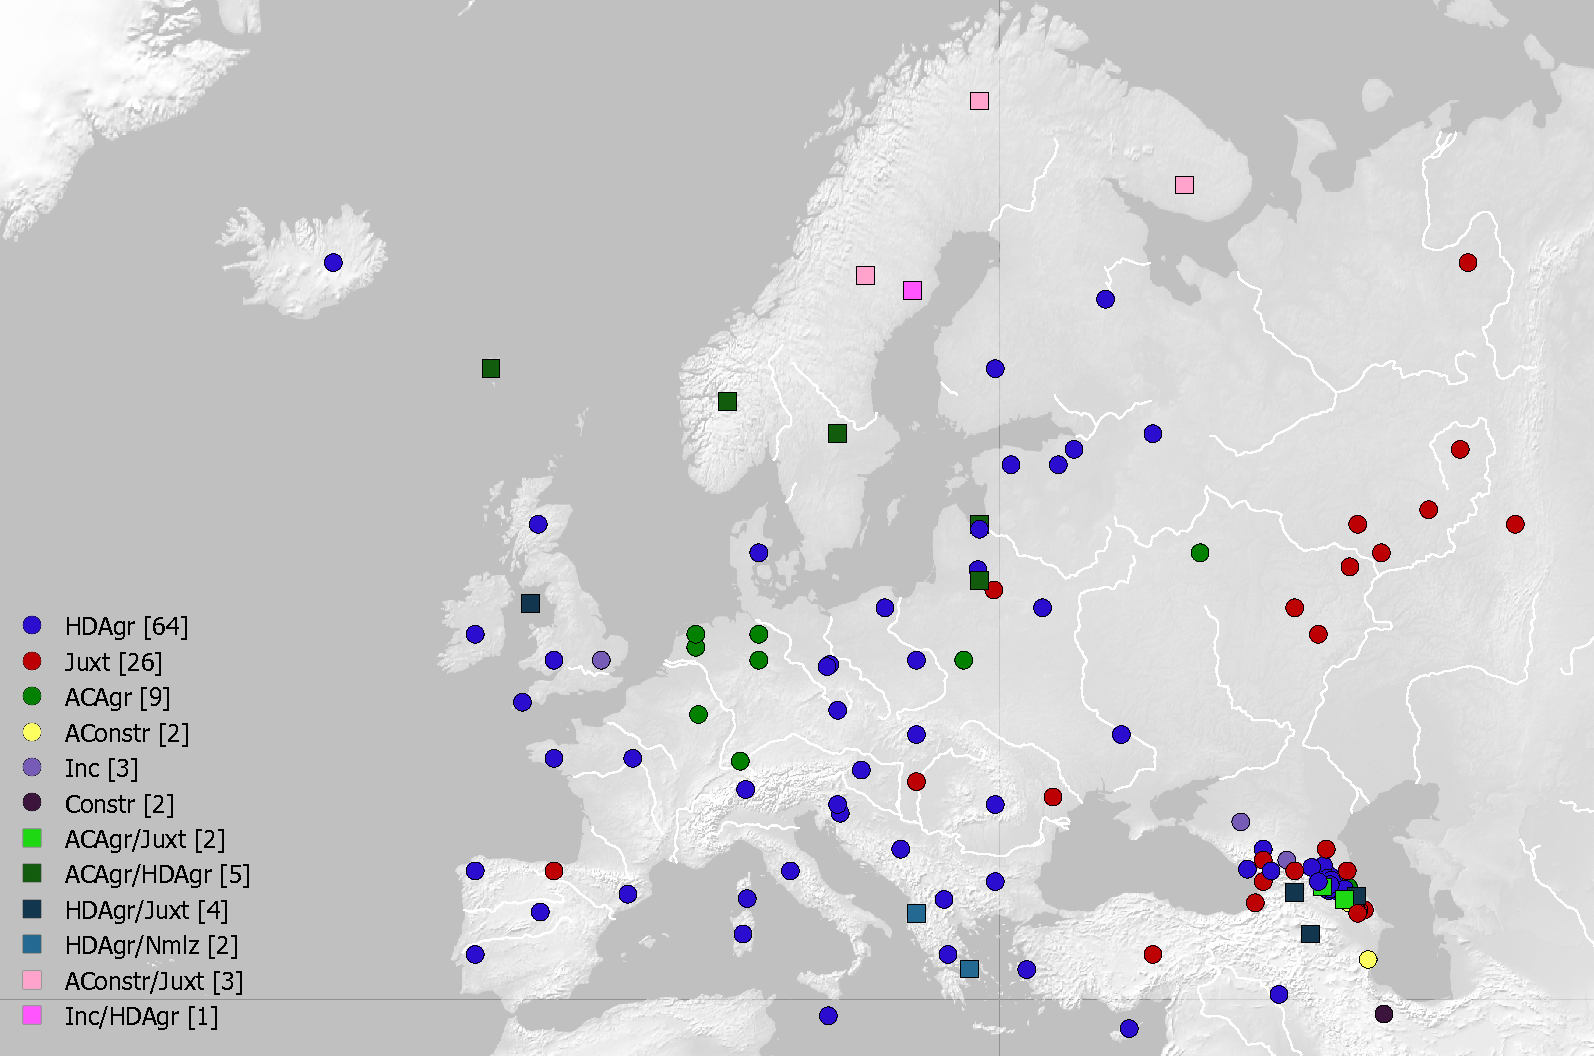
\includegraphics[width=\textheight,angle=90]{EUMap.jpg}
\label{EUMap}
\end{sidewaysfigure}

\newpage
\begin{sidewaysfigure}
    \begin{minipage}[b][8cm][c]{2\baselineskip}
        \caption[Adjective attribution marking, Europe, main types]{Adjective attribution marking in the languages of Europe; 123 languages coded for main morpho-syntactic types}
    \end{minipage}
%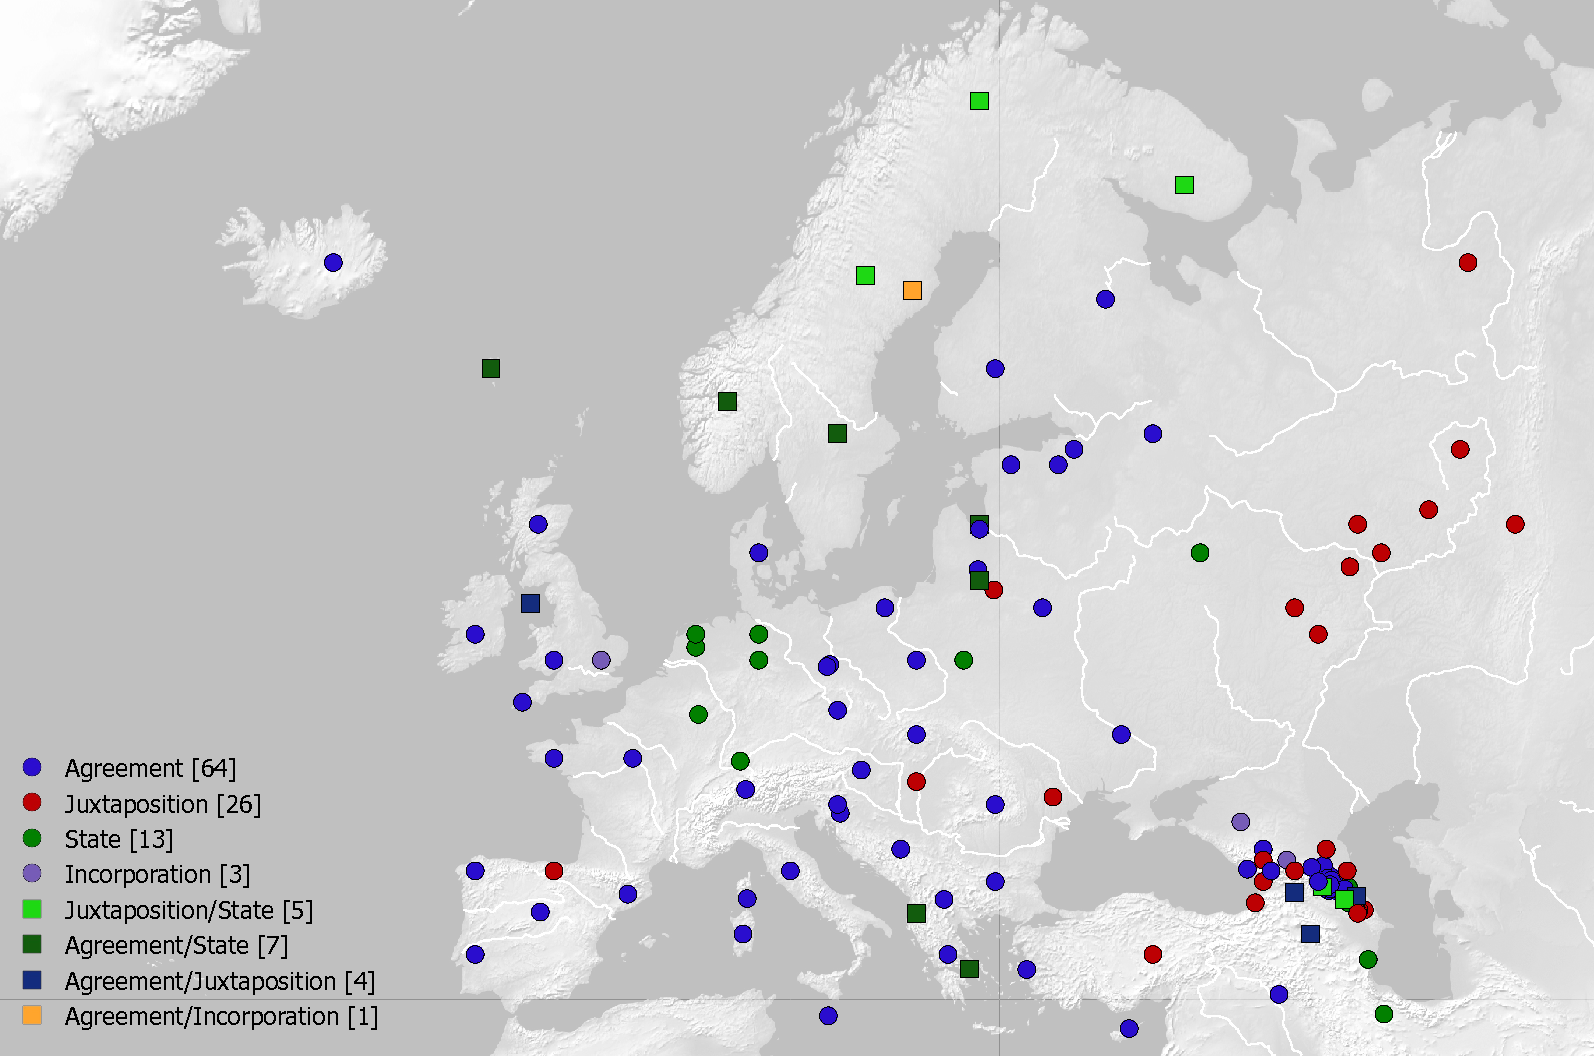
\includegraphics[width=\textheight,angle=90]{EUMapTyp.jpg}
\label{EUMapTyp}
\end{sidewaysfigure}

